\documentclass[12pt,a4paper]{article}
\usepackage[utf8]{inputenc}
\usepackage[francais]{babel}
\usepackage[T1]{fontenc}
\usepackage{amsmath}
\usepackage{amsfonts}
\usepackage{amssymb}
\usepackage{graphicx}
\usepackage{kpfonts}
\author{Mathieu Leocmach}
\title{Memo fractal dimension}
\date{17th December 2014}
\begin{document}

\maketitle

Thanks to Pierre Borgna, things are clearer.

A fractal in a 2D space has the pair correlation function
\begin{equation}
g(r) -1 \sim r^{d-2} e^{-\frac{r}{\xi}}
\end{equation}

To get the structure factor, we Fourier transform in 2D
\begin{align*}
S(q) -1 &\sim \iint e^{-\imath \vec{r}\cdot\vec{q}} \left(g(r)-1\right) \mathrm{d}^2\vec{r}\\
&\sim \int e^{-\frac{r}{\xi}} r^{d-1} \mathrm{d}r
	\int_0^\pi e^{-\imath rq \cos \theta} \sin\theta \mathrm{d}\theta\\
&\sim \int e^{-\frac{r}{\xi}} r^{d-1} 2\frac{\sin qr}{qr}\mathrm{d}r
\qquad\text{by variable change}\qquad X=cos\theta
\addtocounter{equation}{1}\tag{\theequation}\label{eq:exact}\\
\end{align*}

Rather than dig in the involved exact calculus, we just look for a power law in the regime where $q\xi \gg 1$, thus $e^{-\frac{r}{\xi}} \approx 1$ in the integral.
\begin{align*}
S(\lambda q) -1 &\sim \int r^{d-1} 2\frac{\sin \lambda qr}{\lambda qr}\mathrm{d}r\\
&\sim \int \left(\frac{u}{\lambda}\right)^{d-1} 2\frac{\sin qu}{qu}\frac{\mathrm{d}u}{\lambda} \qquad\text{by variable change}\qquad u=\lambda r\\
&\sim \frac{1}{\lambda^d} \left(S(q) -1\right)
\end{align*}

The slope of $S_{2D}(q)$ is thus $-d_{2D}$. Then we suppose that the fractal is isotropic, thus codimension is invariant $2-d_{2D} = 3-d_{3D}$ leading to $d_{3D} = d_{2D}+1$.

\begin{figure}
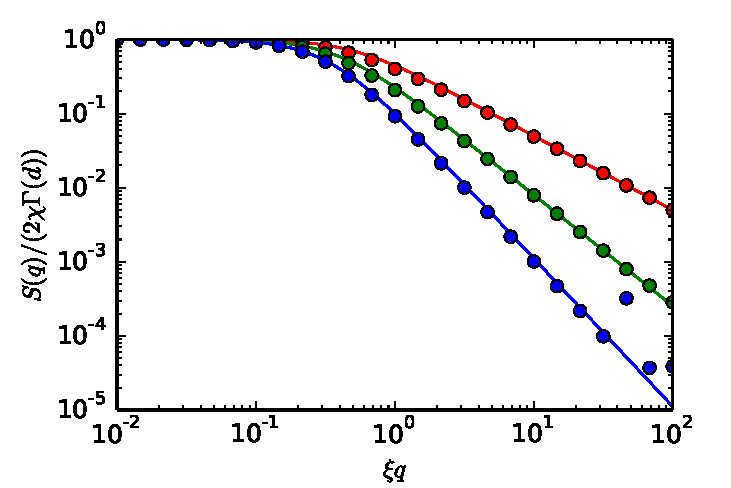
\includegraphics{empirical_fractal}
\caption{Testing empirical expression. Circles are numerical integration of (Eq.~\ref{eq:exact}) normalized by $2\Gamma(d)$ for $d=1,1.5,2$. Lines are the corresponding empirical expression.}
\label{fig:empirical}
\end{figure}

As show in Fig.\ref{fig:empirical} Numerical integration of (Eq.~\ref{eq:exact}) for various $d$ is well fitted by the empirical law:
\begin{equation}
S(q) = \frac{2\chi\Gamma(d)}{\left(1+\left((d+1)\xi q\right)^2\right)^{d/2}}
\end{equation}
where $\chi$ is independent of $d$ and represents the relative contrast between the phases.


\end{document}